% Guidelines on Call for Workshops page at http://www.modelsconference.org

\newif\iflncs
\lncstrue

\iflncs
    \documentclass[runningheads]{llncs}

%
\usepackage{pdfpages}
\usepackage{pbox}
\usepackage[utf8]{inputenc}
\usepackage{url}
\usepackage[T1]{fontenc}
\usepackage{mathabx}
\usepackage[inline]{enumitem}
\usepackage{times}
\usepackage{multirow}

\newcommand{\pcmember}[3]{\item #2 #1, #3}
% comments
\newcommand{\boxedtext}[2]{\colorbox{#1}{\scriptsize\bfseries\textsf{#2}}}
\newcommand{\nota}[3]{
   \boxedtext{#2}{#1}
       {$\blacktriangleright${#3}$\blacktriangleleft$}
}
\newcommand\source[1]{\nota{Source}{green}{#1}}
\newcommand\todo[1]{\nota{TODO}{magenta}{#1}}
\newcommand\placeholder[1]{\textless\textless#1\textgreater\textgreater}
\else
    \documentclass[sigconf, english]{acmart}

\ifxetex
	\usepackage{csquotes}
\else
	\usepackage{babel}
	\usepackage[utf8]{inputenc}
	\usepackage[T1]{fontenc}
\fi

\usepackage{pdfpages}
\usepackage[inline]{enumitem}

% comments
\newcommand{\boxedtext}[2]{\colorbox{#1}{\scriptsize\bfseries\textsf{#2}}}
\newcommand{\nota}[3]{
   \boxedtext{#2}{#1}
       {$\blacktriangleright${#3}$\blacktriangleleft$}
}
\newcommand\source[1]{\nota{Source}{green}{#1}}
\newcommand\todo[1]{\nota{TODO}{magenta}{#1}}
\newcommand\note[1]{\nota{Note}{yellow}{#1}}
\newcommand\placeholder[1]{\textless\textless#1\textgreater\textgreater}


% from https://tex.stackexchange.com/a/346309
\settopmatter{printacmref=false} % Removes citation information below abstract
\renewcommand\footnotetextcopyrightpermission[1]{} % removes footnote with conference information in first column
%\pagestyle{plain} % removes running headers


\usepackage{listings}




\acmConference[MODELS'19]{}{September 2019}{Munich, Germany}
%
\usepackage{pdfpages}
\usepackage{pbox}
\usepackage[utf8]{inputenc}
\usepackage{url}

\newcommand{\pcmember}[3]{\item #2 #1, #3}
\fi

\begin{document}


\title{Third International Workshop on Multi-Paradigm Modeling for Cyber-Physical Systems ({MPM4CPS})}
\iflncs
    \titlerunning{MPM4CPS Workshop Proposal}
\fi

\iflncs
    \author{}
    \institute{}
\else
    \author{Eugene Syriani}
    \affiliation{%
      \institution{Universit\'e de Montr\'eal}
      \country{Canada}
    }
    \email{syriani@iro.umontreal.ca}
    
    \author{Manuel Wimmer}
    \affiliation{%
      \institution{JKU Linz}
      \country{Austria}
    }
    \email{wimmer@big.tuwien.ac.at}
    
    \author{Dominique Blouin}
    \affiliation{%
        \institution{T\'el\'ecom ParisTech}
        \country{France}
    }
    \email{dominique.blouin@telecom-paristech.fr}
    
    \author{Moussa Amrani}
    \affiliation{%
        \institution{Universit\'e de Namur}
        \country{Belgium}
    }
    \email{Moussa.Amrani@unamur.be}
    
    \author{Julien Deantoni}
    \affiliation{%
        \institution{Universit\'e Nice - Sophia Antipolis}
        \country{France}
    }
    \email{julien.deantoni@univ-cotedazur.fr}
    
    \author{Hans Vangheluwe}
    \affiliation{%
      \institution{University of Antwerp - Flanders Make vzw}
    }
    \affiliation{%
        \institution{McGill University}
        \country{Canada}
    }
    \email{hans.vangheluwe@uantwerpen.be}
 
    \author{Pieter Mosterman}
    \affiliation{%
      \institution{The Mathworks}
    }
    \email{Pieter.Mosterman@mathworks.com}
   
    \author{Jeff Gray}
    \affiliation{%
        \institution{University of Alabama }
        \country{USA}
    }
    \email{gray@cs.ua.edu}
    
    \author{Vasco Amaral}
    \affiliation{%\affiliation{%
        \institution{Universidade NOVA de Lisboa}
        \country{Portugal}
    }
    \email{vasco.amaral@fct.unl.pt}
    \renewcommand{\shortauthors}{Van Mierlo, Syriani, Wimmer, Blouin, Amrani, Deantoni, Vangheluwe, Gray, Amaral}
\fi

\maketitle
\iflncs
    \vspace{-1cm}
\fi

\section{General Information}
%\noindent
%\textbf{Title}: $1^{st}$ International Workshop on Multi-Paradigm Modeling for Cyber-Physical Systems \\

%\noindent
%\textbf{Acronym}: MPM4CPS \\

% \begin{tabular}{| c | c | c | c |}
% \hline
% \multicolumn{4}{|c|}{\textbf{MPM4CPS: Preferably Full Day}}\\
% \hline
% \parbox[t]{2mm}{\multirow{6}{*}{\rotatebox[origin=c]{90}{\textbf{Organisers}}}} 
%     & \textbf{Simon Van Merlo} & \begin{tabular}{c}
%         University of Antwerp \\ 
%         Flanders Make 
%     \end{tabular} & {\small \texttt{simon.vanmierlo@uantwerpen.be}} \\
% \cline{2-4}
%     & \textbf{Eugene Syriani} & University of Montréal & {\small \texttt{syriani@iro.umontreal.ca}}\\
% \cline{2-4}
%     & \textbf{Manuel Wimmer}  & JKU Linz, CDL-MINT & {\small \texttt{manuel.wimmer@jku.at}}\\
% \cline{2-4}
%     & \textbf{Dominique Blouin} & Télécom ParisTech& {\small \texttt{dominique.blouin@telecom-paristech.fr}}\\
% \cline{2-4}
%     & \textbf{Moussa Amrani} & Université de Namur & {\small \texttt{Moussa.Amrani@unamur.be}}\\
% \cline{2-4}
%     & \textbf{Julien Deantoni} & Université Nice - Sophia Antipolis & {\small \texttt{julien.deantoni@univ-cotedazur.fr}}\\
% \hline\hline
% \parbox[t]{2mm}{\multirow{4}{*}{\rotatebox[origin=c]{90}{\textbf{Steering }}}} 
%     & \textbf{Hans Vangheluwe} & \begin{tabular}{c}
%         University of Antwerp\\
%         Flanders Make\\
%         McGill University
%     \end{tabular} & {\small \texttt{hv@cs.mcgill.ca}}\\
% \cline{2-4}
%     & \textbf{Jeff Gray} & University of Alabama & {\small \texttt{gray@cs.ua.edu}}\\
% \cline{2-4}
%     & \textbf{Vasco Amaral} & Universidade NOVA de Lisboa & {\small \texttt{vasco.amaral@fct.unl.pt}}\\
% \hline
% \end{tabular}

\noindent
\textbf{Organizers}:\\
\textbf{Moussa Amrani}, (primary contact) University of Namur, moussa.amrani@unamur.be\\
\textbf{Dominique Blouin}, T\'el\'ecom Paris, Institut Polytechnique de Paris, dominique.blouin@telecom-paris.fr\\
\textbf{Moharram Challenger}, University of Antwerp - Flanders Make, moharram.challenger@uantwerpen.be\\
\textbf{Julien Deantoni}, Universit\'e Nice - Sophia Antipolis, julien.deantoni@univ-cotedazur.fr\\
\textbf{Robert Heinrich}, Karlsruhe Institute of Technology (KIT), robert.heinrich@kit.edu\\
\textbf{Manuel Wimmer}, JKU Linz, CDL-MINT, manuel.wimmer@jku.at

\bigskip
\noindent
\textbf{Steering Committee}:\\
\textbf{Hans Vangheluwe}, University of Antwerp – Flanders Make, hv@cs.mcgill.ca\\
\textbf{Pieter J. Mosterman}, The Mathworks, Pieter.Mosterman@mathworks.com\\
\textbf{Jeff Gray}, University of Alabama, gray@cs.ua.edu\\
\textbf{Vasco Amaral}, Universidade NOVA de Lisboa, vasco.amaral@fct.unl.pt\\


\noindent
\textbf{Desired Length of the Workshop}: Full Day \\

\noindent
\textbf{Abstract}: 
\begin{small}
The networked combination of multi-physics systems (mechanical, 
electrical, hydraulic, biochemical, among others) with computational systems 
(control systems, signal processing, logical inference, planning, among others), 
often interacting with human actors, in uncertain environments, in a socio-economic 
context, has led to so-called Cyber-Physical Systems (CPS).
The CPS that are engineered today are reaching a previously unseen level of 
complexity.
To date, no unifying theory nor systematic design methods, techniques and tools 
exist for such systems.
Individual (mechanical, electrical, network or software) engineering disciplines 
only offer partial solutions.
Multi-Paradigm Modeling (MPM) proposes to \emph{model} every part and aspect of 
such complex systems \emph{explicitly}, at the most appropriate level(s) of 
abstraction, using the most appropriate modeling formalism(s).
This includes the explicit modeling of the often complex engineering workflows.
Modular modeling language engineering, including model transformation and the 
study of modeling language semantics, are used to realize MPM, which has the 
potential to be an effective answer to the challenges of designing CPS.
This third edition is aimed at furthering the state-of-the-art as well as 
defining the future directions of this emerging research area by bringing together 
international experts in the field for an intense one-day workshop.
\end{small}

\section{Objectives and Scope}

\subsection{Motivation}
Tackling the complexity involved in developing truly complex, designed systems 
is a topic of intense research and development.
In the past, system complexity has drastically increased once software components 
were introduced in the form of embedded systems, controlling physical parts of 
the system, and has only grown in CPS, where the networking aspect of the systems 
and their environment are also taken into account.
The complexity faced when engineering CPS is mostly due to the plethora of 
cross-disciplinary design alternatives and inter-domain interactions.
To date, no unifying theory nor system design methods, techniques, or tools to 
design, analyze, and ultimately deploy CPS exist.
Individual (physical systems, network, software) engineering disciplines offer 
only partial solutions and are no match for the complexity observed in CPS.
Multi-Paradigm Modeling (MPM) offers a foundational framework for gluing the 
several disciplines together in a consistent way.
The inherent complexity of CPS is broken down into different levels of 
abstraction and views, each expressed in appropriate modeling formalisms.
MPM offers processes and tools that can integrate the views, abstractions and 
components that make up a CPS.\\
MPM encompasses many research topics: from language engineering (for DSLs, 
including their (visual) syntax and semantics), to processes to support multi-view 
and multi-abstraction modelling, simulation for full-system analysis, and deployment.
The added complexity that CPS bring compared to embedded and software-intensive 
systems requires consideration of how MPM techniques can be applied or adapted 
to these new applications, tying together multiple domains.
Many remaining research questions require answers from researchers in different 
domains, as well as a unified effort from researchers that work on supporting 
techniques and technologies.
The community needs a workshop setting to meet up and align past and future 
research activities.

%Topics of interest include:
%\begin{itemize}
%    \item Foundations of domain-specific modeling with a particular focus on ``blended'' textual/visual modeling and the modeling/formal analysis/simulation/synthesis of complex user interfaces.
%    \item Modeling language engineering, modular design of modeling languages.
%    \item Co-simulation, coordination algorithms ensuring correct simulation results.
%    \item Digital twins of complex systems and their relationship to MPM techniques.
%    \item Applications of MPM techniques in automotive, aviation, manufacturing, \ldots
%    \item MPM for (self-)adaptive systems
%    \item Machine learning applied in an MPM context
%\end{itemize}

\subsection{Objectives}
The purpose of this workshop is to bring together researchers and practitioners 
in the area of MPM (specifically applied to developing CPS) in 
order to identify possible points of synergy, common problems and solutions, 
tool building aspects and the vision for the future of the area.
The goal is to organize a highly interactive workshop. A significant portion of 
the Workshop will be dedicated to \textbf{discussions}. \textbf{"Regular" Research 
papers} from academic and industry authors will present novel research results 
on the Workshop's topics of interest. We will encourage the submission of 
out-of-the-box presentations, which are not deeply researched yet, but can lead 
to new insights, discussions, and future collaborations.
\textbf{"Lightning Talks"}, submitted in the form of a two-page papers following
the recommended format, not published in the proceedings, will foster discussions
and encourage interactions between participations. 
We will invite the submission of \textbf{Exemplars}, i.e., typical yet relatively
tractable use cases of CPS systems demonstrating typical activities required for
CPS Engineering, and explicitly detailing the underlying formalisms, languages and
tools deployed to support such activities, all expressed in a similar way to enable
comparison and extract CPS Engineering common practices and design patterns.


\subsection{Context}
The MPM community has been actively researching new techniques for system design 
for over a decade, through many related events.
One-week Computer Automated Multi-Paradigm Modeling (CAMPaM) workshops have been 
organized yearly since 2004 at McGill University’s Bellairs campus, Barbados. 
Additionally, the International Summer School on Domain-Specific Languages - 
Theory and Practice (DSM-TP), focused on the education of language engineering 
techniques, and has been organized since 2009.
Its target audience includes Ph.D. students, researchers, and software industry 
professionals.
Most recently, a European Cooperation in Science and Technology (COST) research 
network has been active since 2015 on the use of MPM techniques for designing 
CPS, bringing together 29 European partner countries\footnote{https://www.cost.eu/actions/IC1404/ 
and http://mpm4cps.eu/}.
The chair and co-chair of this network (Hans Vangheluwe and Vasco Amaral) are 
members of the steering committee for this workshop.
The first edition of the workshop has lead to the preparation of a theme section on the topic of MPM4CPS for the SoSyM journal (which has been recently published\footnote{ https://link.springer.com/article/10.1007/s10270-021-00882-1}).
These initiatives demonstrate both the continued relevance of the topic and the 
potential impact of the workshop.


%\subsection{Topics of Interest}
\subsection{Intended Audience}
The intended audience includes researchers as well as practitioners who are 
interested in MPM techniques in the context of CPS development.
We expect to attract many attendees of earlier MPM-related events, those who 
contributed to the COST action, as well as a broader audience.
This encompasses researchers that work on the fundamentals of language 
engineering, (visual) modeling environment construction, (co-)simulation 
techniques, as well as tool builders and users of these tools.
The MODELS conference is an ideal venue for organizing MPM4CPS since it brings 
together researchers that aim to advance the state-of-the-art in model-driven 
engineering and practitioners who have valuable application experiences to share.

\subsection{Need}
The MPM4CPS workshop (series) follows the successful series of nine MPM workshops that 
were organized as part of the MODELS conference during the years 2006 through 2015.
These workshops attracted many participants in the past, and we saw that the topic
is still relevant, since the previous editions attracted many submissions and lively discussions.
These two reasons make this workshop worth organizing at MODELS this year.

Historically, GeMoC and EXE, now merged into the MLE (Modeling Language 
Engineering and Execution), were the closest workshops planned to be organised 
in MoDELS this year. They focus mainly on two topics: the globalization of
modeling techniques, which include techniques and processes to create and
integrate heterogeneous languages, and the execution, animation and debugging
of modeling languages. While both are concerned with specific aspects of 
\emph{software} language engineering, MPM includes modeling languages for 
physical domains (e.g., electrical, mechanical, etc.) that require 
continuous-time solvers for simulation, and clean integration with other (SW/HW) 
languages.
MPM4CPS further differentiates from those workshops by focusing on CPS. 
We believe that both workshops can strengthen each other by focusing on different 
(specialized) aspects of challenges within the MODELS community.

%MDE4IoT addresses the challenges in creating and managing a highly dynamic network 
%of systems.
%Although similar from an abstract viewpoint (``things'' may be computer-based or 
%physical objects), the MDE4IoT workshop is highly specialized and investigates 
%how MDE techniques can be used to develop the networking aspect of IoT applications, 
%shifting the focus on (SW) architecture and abstracting away from the physical 
%properties of ``thing'', which sets MPM4CPS apart.

The challenges to design and develop CPS, with a focus on MPM techniques as a 
foundational framework for supporting the multi-domain models, tools, and 
processes are fundamental enough to warrant a focused workshop.

\section{Organization Details}
%\subsection{Organizers}
\noindent
\textbf{Moussa Amrani} obtained his Ph.D. in 2013 from the University of Luxembourg. 
He is currently a postdoctoral researcher at the University of Namur and the Namur Digital Institute in Belgium. 
He is (co-)author of over 50 papers on MDE, IoT and formal verification published in international conferences (MODELS, SLE, ECMFA, ASE, ETAPS, NFM, CAiSE, \ldots) and journals (SoSyM, JSS, TSE, ToSEM, JoT, IST, ComLan, \ldots). He co-founded and co-organized the VoLT workshop at MoDELS from its inception in 2013, and co-organised
the previous editions of the MPM4CPS Workshop.

\noindent
\textbf{Dominique Blouin} is a research engineer at Telecom Paris, Institut Polytechnique Paris 
(France). He obtained an M.Sc. in Physics (Canada) and a Ph.D. in Computer Science (France) in 2013. He worked for many years in industry as a software architect and was the vice-chair of the Foundational Aspects Working Group in the MPM4CPS COST Action. He has been an active member of the SAE AADL standardization committee for the past 10 years. His research interests are MPM, model management, model transformation and (bi-directional) synchronization, requirements engineering, CPS.

\noindent
\textbf{Moharram Challenger} is a research professor at the University of Antwerp, Belgium. He was the CTO of a software company involved-in/leading several national or international software intensive projects. He has served as an organisation committee member for SummerSim'20, ICSMM'20, AnnSim'21, IWCPS@FedCSIS'21, and AMSC'21. Also, he played the role of co-chair for several workshops organised in MoDELS and STAF 2020-21 (MDE-Intelligence, MPM4CPS, MDE4IoT, SERP4IoT, SEDES, MESS, EMAS, etc.)

\noindent
\textbf{Julien Deantoni} obtained his Ph.D. in 2007 from INSA Lyon, France. He is currently an Associate Professor at University of Côte d'Azur in Nice Sophia-Antipolis, France and associated with the Kairos research team (INRIA \& I3S).
% received a Ph.D. degree in Computer Science from the INSA--Lyon engineering school, France in  2007. His Ph.D was realized in the embedded systems team of the CITI laboratory from 2004 to 2007 where he successfully participated to international robotic challenges to highlight the  benefits of model driven analysis. After having a postdoctoral fellow (funded by the  European SPEEDS project) in the Triskell team at INRIA Rennes, he is currently associate  professor at University of Cote d'Azur and a member of the Kairos project-­team (INRIA \& I3S). 
His research interest concerns the use and the definition of formal methods and tools for MDE.
%More information is available at \url{http://www.i3s.unice.fr/~deantoni/}. His experience as organizer are:
He served as track-chair at the Computational science track at IEEE RIVF'19, co-chair of the GeMoC Workshop series hosted at MODELS (2013--2017), chair of the Doctoral Symposium at the Summer School on Real-Time Systems (2007) and co-organizer of a Specific Action on Heterogeneity from Modeling until Simulation in 2011.

\noindent
\textbf{Robert Heinrich} holds a Ph.D. from Heidelberg University, and is head of the Quality-driven System Evolution research group at KIT. His research interests include modularization
and composition of model-based analysis for performance, confidentiality and maintainability, etc. applied to information systems, business processes and automated production systems. One core asset of his work is the Palladio software architecture simulator. He is involved in the organization committees of several international conferences, established and organized various workshops, is reviewer for international premium journals (IEEE TSE and IEEE Software), and academic funding agencies.


\noindent
\textbf{Manuel Wimmer} is full professor at the Department of Business Informatics - Software Engineering at JKU Linz, Austria and is the head of the Christian Doppler Laboratory CDL-MINT. %He received his Ph.D. and his Habilitation from TU Wien. He has been a research associate at the University of Malaga and a visiting professor at the University of Marburg as well as at TU Munich. 
He is/was involved in several national and international projects dealing with the application of model engineering techniques for domains such as tool interoperability, versioning, Cloud computing, IoT, and factory and building automation. 
%He is coauthor of the book Model-driven Software Engineering in Practice (Morgan \& Claypool, 2nd edition, 2017) and coauthor of more than 200 scientific articles published in international conferences (e.g., MODELS, ASE, ICMT, ECMFA) and journals (e.g., ACM CSUR, SoSyM, JSS, ASE, TSE, IST). 
He has served as PC co-chair for ICMT'15, SEAA'20, workshop co-chair for ICWE'12, STAF'16 and MODELS'16, track co-chair for ICWE'14, CBI'18 and SEAA'17--19, poster co-chair for MODELS'14 and ICWE'16, and organized MDWE'13, VOLT'13--15, CMSEBA'14, MULTI'17\&19--20, MDEbug'17--18, PNSE'19, MDE Intelligence'19--20, MPM4CPS'19--20, and MDE4IoT'17--20.
% \iflncs
%     \begin{itemize*}
%         \item Track-chair of the Computational science track of the IEEE RIVF 2019 conference.
%     	\item Co-chair of the several International Workshops on the Globalization of Modeling Languages @ MODELS 2013/2014/2015/2016/2017 (GEMOC'xx)
%     	\item Chair of the doctoral symposium at the summer school on real time systems (2007)
%     	\item Co-organizer of a national meeting on heterogeneity from modeling until simulation in 2011 (\url{http://gemoc.org/as2011/})
%     \end{itemize*}
% \else
%     \begin{itemize}
%         \item Track-chair of the Computational science track of the IEEE RIVF 2019 conference.
%     	\item Co-chair of the several International Workshops on the Globalization of Modeling Languages @ MODELS 2013/2014/2015/2016/2017 (GEMOC'xx)
%     	\item Chair of the doctoral symposium at the summer school on real time systems (2007)
%     	\item Co-organizer of a national meeting on heterogeneity from modeling until simulation in 2011 (\url{http://gemoc.org/as2011/})
%     \end{itemize}
% \fi

\subsection{Program committee: to be contacted, cf. CfP in Appendix}

\subsection{Possibility to merge with another workshop}
We request that MPM4CPS be run on its own and we plan half a day of discussions.
We can merge with another workshop if this is a condition from the organization 
and the topics are similar enough.

\section{Workshop Format}
\subsection{Planned Deadlines \& Intended Paper Format: cf. CfP in appendix}

\subsection{Evaluation Process}
At least three reviewers will evaluate each submission.
Full research papers will be reviewed using standard scientific criteria: alignment 
with the workshop topic(s), novelty, evaluation, and ability to generate discussion.
Short papers and extended abstracts will be evaluated based on their likelihood 
to spark lively discussions at the workshop.

\subsection{Intended Workshop Format}
The Workshop will include keynotes, ideally one from academia and the other from industry
(depending on how people are available). A morning keynote will set the stage for the
rest of the day, followed by paper presentations. A second keynote after the lunch break
will set the discussion around exemplar presentations and lightning talks, which will
foster discussions and out-of-the-box ideas.
Talks throughout the day will be followed by discussions. The afternoon will reserve
time to discuss the examplars, by starting discussions around identifiable patterns,
common practices, popular formalisms/languages/tools, etc. 
The workshop will end with a wrap-up discussion to formulate the workshop's 
conclusion, identify open challenges, and outline future work.
A summarizing publication will be included in the proceedings.

\subsection{Number of expected participants: 25-35 (similar to last year's virtual ed.)}

\subsection{Equipment: Virtual Room with shared virtual blackboard}

\section{Additional Material}

\textbf{See Appendix} for \textbf{Draft Call for Papers} \& \textbf{Webpage}



\newpage
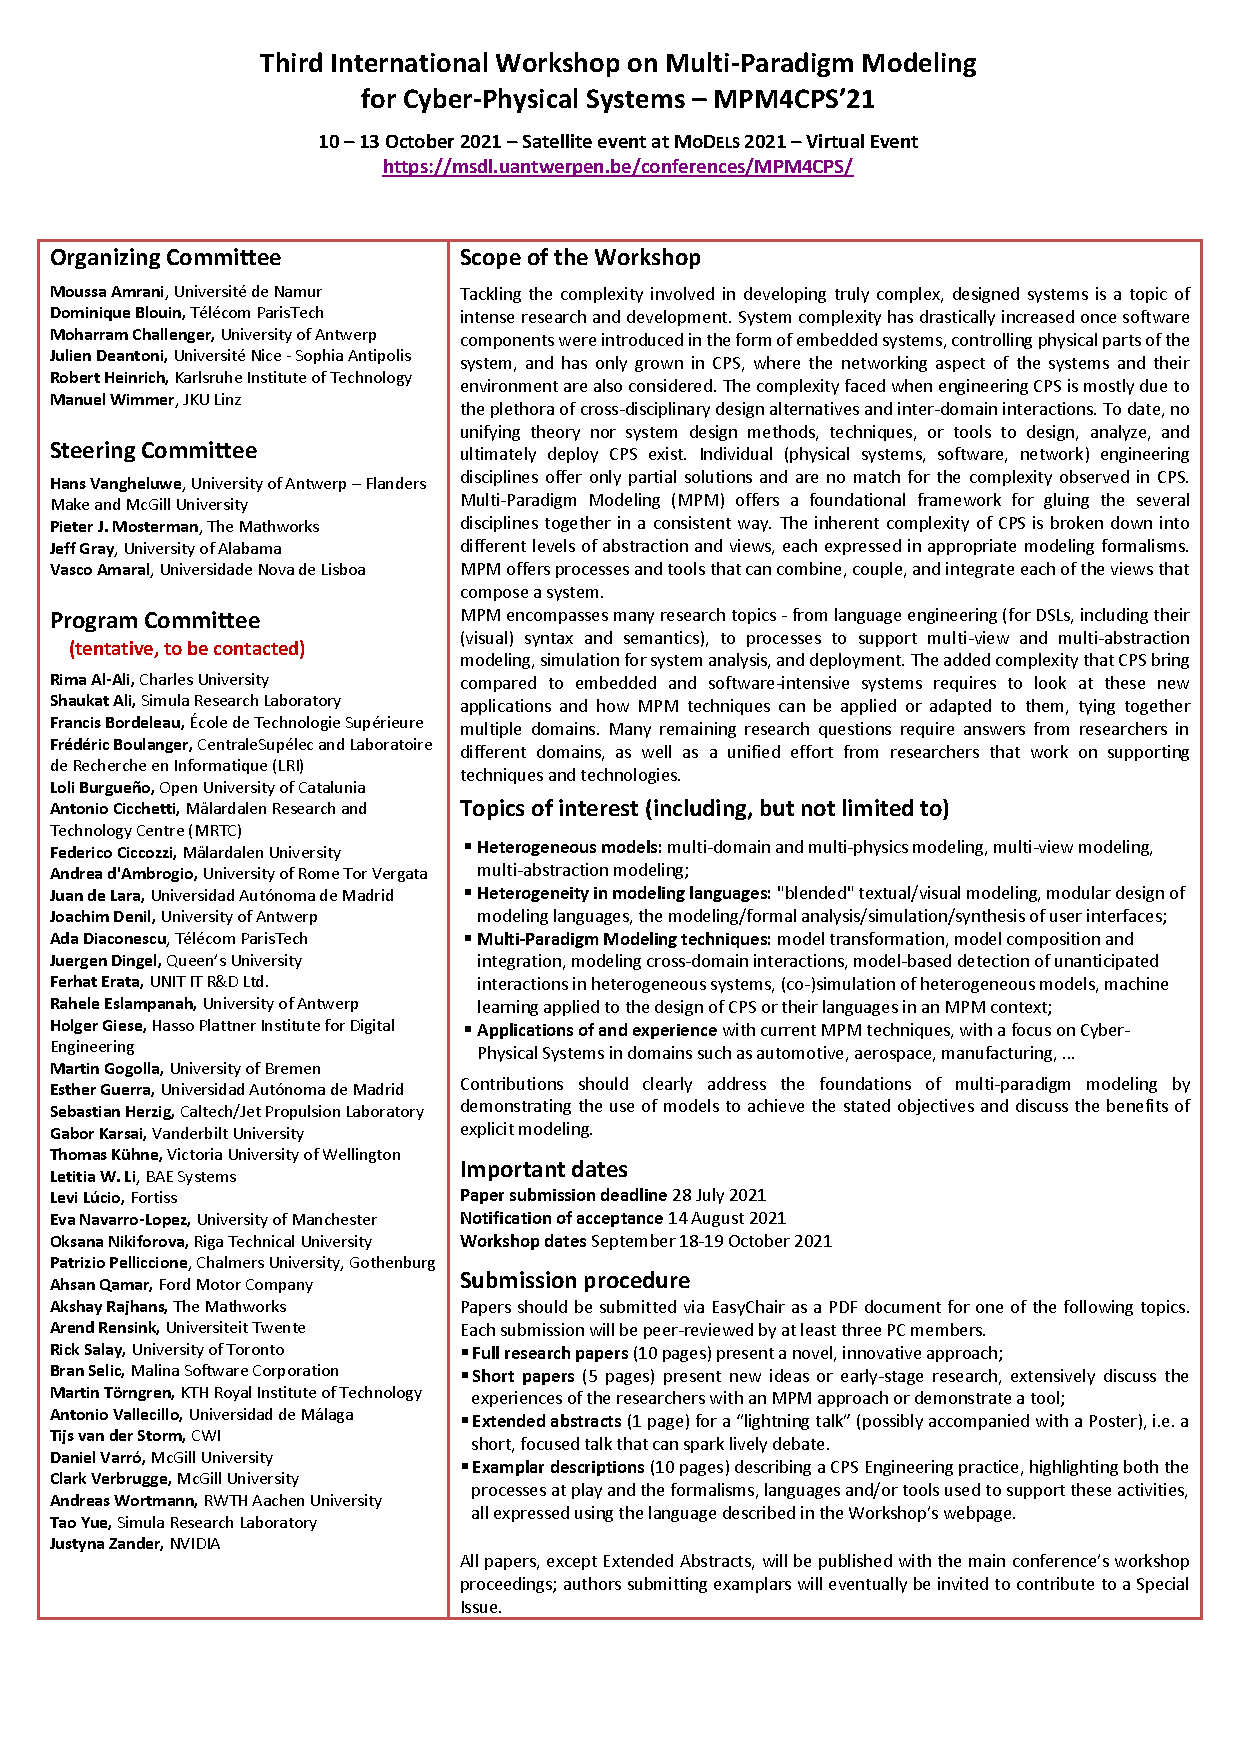
\includepdf{MPM4CPS21-CfP.pdf}

\end{document}